% Use style package recommended by conference.
\documentclass[letterpaper,single,9pt]{article}

\usepackage[all=normal, paragraphs, indent, lists, floats, sections, title]{savetrees}

\usepackage{epsfig}
\usepackage{graphicx}
\usepackage{subfigure}
\usepackage{amsmath,amssymb}
\usepackage{color}
\usepackage[hyphens]{url}
\usepackage{listings}
\usepackage[normalem]{ulem}
\usepackage{floatrow}
\usepackage{xspace}
\usepackage{amsmath}
\usepackage{enumitem}
\usepackage{booktabs}
\usepackage[utf8]{inputenc}
\usepackage{authblk}
\usepackage{hyperref}
\usepackage{algorithm, algpseudocode}
\usepackage{fancyvrb}
\usepackage{cprotect}
\usepackage{mdframed}
\usepackage{array}
\usepackage{cite}
\usepackage{multirow}
\usepackage{caption}
\usepackage[usenames,dvipsnames]{xcolor}
\renewcommand{\theenumi}{\Alph{enumi}}
\begin{document}
\title{COMS W4771 - Machine Learning 4th Exersice}

  \author{ {\rm Georgios Koloventzos - gk2409} \\ }

\maketitle

%\section*{Problem 1}
The EM algorithm for multinomial distributions is similar to the Gaussian ones.
I will use the steps that are also depicted in Bishop's book in chapter 9 for
Gaussian.
\begin{align*}
p(x) = \sum_{k=1}^K \pi_k p(x \mid \mu_k)
\end{align*}
also
\begin{align*}
\pi_k p(x \mid \mu_k) = \prod_{j=1}^M \mu_k (j)^{x(j)}
\end{align*}
The $z$ values (mixing coeffient) of having the same properties of Gaussian mixtures.
So the $p( z_k = 1) = \pi_k$ for which $\sum_{k=1}^k \pi_k = 1$
The marginal distribution $p(z)$ can be written as:
\begin{align*}
p(z) = \sum_{k=1}^K \pi_{k}^(z_k)
\end{align*}
and
\begin{align*}
p(x_j =1 \mid z=k) = p(x\mid z=k) \mu_l
\end{align*}
Using this equations we have 
\begin{align*}
p(x\mid z) = \prod_{k=1}^K (\mu_{k})^ z_{k}
\end{align*}
So combining all these:
$p(x) = \sum_{k=1}^K p(z)p(x\mid z) = \sum_{k=1}^K \pi_k \mu_k$
\subsection*{E-step}
For the E step we have to calculate the $t_nj$ as we see in the problem statement.
By Bayes' Rule we have
$t_nj=p(z_n =j \mid x_n,\theta) = p(z_n =j)p(x\mid z_n,\theta)$
if we plug the densities we already have:
\begin{align*}
p(z_n =j \mid x_n,\theta) = \frac{\pi_j \cdot \mu_j}{\sum_{l=1}^K \pi_l \mu_l}
\end{align*}
\subsection*{M-step}
Using the $t$ from E-step we will re-calculate our model $\theta$.
$t_nj=\frac{\pi_j \cdot \mu_j}{\sum_{l=1}^K \pi_l \mu_l}$
So $\theta_j = \frac{\sum_{i=1}^n x_{i} t_i}{M\sum_{i=1}^n t_{i}}$.



%\section{Problem 2}

%\section*{Problem 3}
My implementation of K-means starts with randomly assign K centroids.
Then for each pixel I found the eucleidian distance between the centers
and the pixel. Then I add the pixel to the Kth minimum distance element
in order after dividing this with the number of points on this cluster to
get the new center. The code can be found in problem3.m. It has as an
argument the number of clusters it should produce. It returns the number
of clusters with at least a pixel in.
\begin{figure}[ht] 
  \begin{subfigure}[b]{0.5\linewidth}
    \centering
    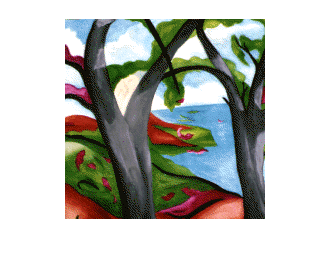
\includegraphics[width=0.75\linewidth]{figures/initial.png}
    \caption{Initial image} 
    \vspace{4ex}
  \end{subfigure}%% 
  \begin{subfigure}[b]{0.5\linewidth}
    \centering
    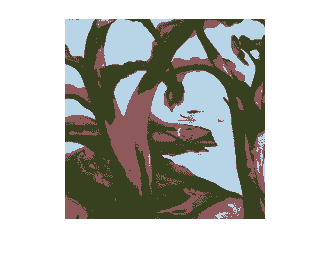
\includegraphics[width=0.75\linewidth]{figures/kmeans3.png} 
    \caption{K=3 clusters}
    \vspace{4ex}
  \end{subfigure} 
  \begin{subfigure}[b]{0.5\linewidth}
    \centering
    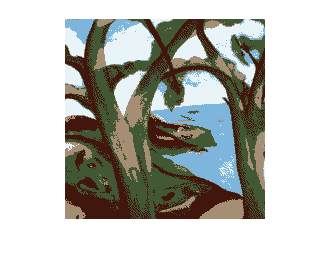
\includegraphics[width=0.75\linewidth]{figures/kmeans5.png}
    \caption{K=5 clusters} 
  \end{subfigure}%%
  \begin{subfigure}[b]{0.5\linewidth}
    \centering
    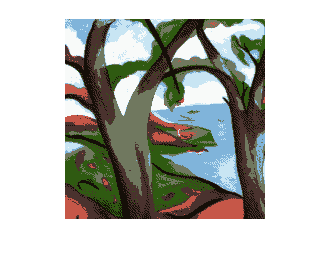
\includegraphics[width=0.75\linewidth]{figures/kmeans8.png} 
    \caption{K=8 clusters} 
  \end{subfigure} 
  \caption{Illustration of various K-means clustering}
\end{figure}

For the initialization and inconsistencies:
Picking random points as initialization points can lead to empty or weird clusters. Specifying
more clusters as you can handle can create empty ones (if you run my program with 20 you will get
only 17 clusters) or the ones that will be created are not distinct. Picking pixels form the image
can lead to inconsistencies also as you may pick an outlier that will not have any point as cluster.
Also picking some specific ones (I had done some experiments with 3 clusters(Red, Green, Blue) or 5
(the previous plus Black and White)) but I did not had any better result. 

In order to solve this problem the community chooses either to run multiple time the K-means and
pick the best. But still this technique is not guaranteed. Other are running other cluster algorithms
like hierarchical in order to get some good initial points. Another solution is to remove outliers
in order to pick some more consistent centroids. A wide applicable approach as the problem is NP-hard
is the K-means++ algorithm. Matlab's kmeans function is using the k-meams++ algorithm.

%%\clearpage{}
\section*{Problem 4}
\subsection*{a)}
The arithmetic mean of non-negative numbers is at least their geometric mean:
\begin{align*}
\frac{x_1 + x_2 + \cdots + x_n}{n} \geq \sqrt[n]{x_1 \cdot  x_2  \cdots x_n}
\end{align*}
Jensen's inequality for concave function is:
\begin{align*}
f\bigg(\frac{\displaystyle\sum_{i=1}^{n}x_i}{n}\bigg) \geq \frac{\displaystyle\sum_{i=1}^{n}f(x_i)}{n}
\end{align*}
Also we know that $f(x) = \log(x)$ is concave for $x > 0$. So we can infer:
\begin{align*}
\log\bigg(\frac{\displaystyle\sum_{i=1}^{n}x_i}{n}\bigg) \geq \frac{\displaystyle\sum_{i=1}^{n}\log(x_i)}{n} \Leftrightarrow \\
\log\bigg(\frac{x_1 + x_2 + \cdots + x_n}{n}\bigg) \geq \frac{\log\displaystyle\prod_{i=1}^{n}(x_i)}{n} \Leftrightarrow \\
\log\bigg(\frac{x_1 + x_2 + \cdots + x_n}{n}\bigg) \geq \log\displaystyle\prod_{i=1}^{n}(x_i)^\frac{1}{n}
\end{align*}
As the log function is always increasing then we can remove the log without changing inequality direction.
We then have:
\begin{align*}
\bigg(\frac{x_1 + x_2 + \cdots + x_n}{n}\bigg) \geq \displaystyle\prod_{i=1}^{n}(x_i)^\frac{1}{n} = \sqrt[n]{x_1 \cdot  x_2  \cdots x_n}
\end{align*}
And that is what we wanted to proof.
\subsection*{b)}
For this part we will use general Jensen's equality:
\begin{align*}
f\bigg(\frac{\displaystyle\sum_{i=1}^{n}a_i \cdot x_i}{\displaystyle\sum_{i=1}^{n}a_i}\bigg) \geq \frac{\displaystyle\sum_{i=1}^{n}a_i\cdot f(x_i)}{\displaystyle\sum_{i=1}^{n}a_i}
\end{align*}
Our goal is to prove:
\begin{align}\label{eq:one}
\displaystyle\sum_{i=1}^{m}exp(\theta^T f_i) \geq exp(\theta^T \displaystyle\sum_{i=1}^{m}a_i f_i - \displaystyle\sum_{i=1}^{m}a_i\log a_i)
\end{align}
where:\\
%$a_i = \frac{exp(\hat{\theta}^T f_i)}{\sum_{i=1}^{m}exp(\hat{\theta}^T f_i)}$\\
One first reliazation is that the summation of $a_i$ is equal to 1:
\begin{align*}
\displaystyle\sum_{i=1}^{n}a_i = \frac{\displaystyle\sum_{i=1}^{n}exp(\hat{\theta}^T f_i)}{\displaystyle\sum_{i=1}^{m}exp(\hat{\theta}^T f_i)}
\end{align*}
Also we can infer that $a_i < 1$ sincewe divide with a normalization constant.\\

So for the left side of our inequality ~\ref{eq:one}, we can write it as:
\begin{align}\label{eq:left1}
\displaystyle\sum_{i=1}^{m}exp(\theta^T f_i) = \frac{\displaystyle\sum_{i=1}^{m}exp(\theta^T f_i)}{\displaystyle\sum_{i=1}^{m}a_i} \geq \frac{\displaystyle\sum_{i=1}^{m}a_i exp(\theta^T f_i)}{\displaystyle\sum_{i=1}^{m}a_i}
\end{align}
Combining ~\ref{eq:one} and ~\ref{eq:left1} we get
\begin{align*}
\frac{\displaystyle\sum_{i=1}^{m}a_i exp(\theta^T f_i)}{\displaystyle\sum_{i=1}^{m}a_i} \geq exp(\theta^T \displaystyle\sum_{i=1}^{m}a_if_i - \displaystyle\sum_{i=1}^{m}a_i\log a_i)
\end{align*}
Now having this can we solve as:
\begin{align*}
\frac{\displaystyle\sum_{i=1}^{m}a_i exp(\theta^T f_i)}{\displaystyle\sum_{i=1}^{m}a_i} \geq exp(\theta^T \displaystyle\sum_{i=1}^{m}a_i f_i - \displaystyle\sum_{i=1}^{m}a_i\log a_i) \Leftrightarrow \\
\frac{\displaystyle\sum_{i=1}^{m}a_i exp(\theta^T f_i)}{\displaystyle\sum_{i=1}^{m}a_i} \geq exp(\displaystyle\sum_{i=1}^{m}\theta^T a_i f_i - \displaystyle\sum_{i=1}^{m}a_i\log a_i) \Leftrightarrow \\
\frac{\displaystyle\sum_{i=1}^{m}a_i exp(\theta^T f_i)}{\displaystyle\sum_{i=1}^{m}a_i} \geq \frac{exp(\displaystyle\sum_{i=1}^{m}\theta^T a_i f_i)}{exp(\displaystyle\sum_{i=1}^{m}a_i\log a_i))} \Leftrightarrow \\
\frac{\displaystyle\sum_{i=1}^{m}a_i exp(\theta^T f_i)}{\displaystyle\sum_{i=1}^{m}a_i} \geq \frac{exp(\displaystyle\sum_{i=1}^{m}a_i\theta^T f_i)}{exp(\displaystyle\sum_{i=1}^{m}a_i\log a_i))} \Leftrightarrow \\
\frac{\displaystyle\sum_{i=1}^{m}a_i exp(\theta^T f_i)}{\displaystyle\sum_{i=1}^{m}a_i} \geq \frac{exp(\displaystyle\sum_{i=1}^{m}a_i\theta^T f_i)}{exp(\displaystyle\sum_{i=1}^{m}(\log a_i)^{a_i}))} \Leftrightarrow \\
\frac{\displaystyle\sum_{i=1}^{m}a_i exp(\theta^T f_i)}{\displaystyle\sum_{i=1}^{m}a_i} \geq \frac{exp(\displaystyle\sum_{i=1}^{m}a_i\theta^T f_i)}{\displaystyle\prod_{i=1}^{m}exp((\log a_i)^{a_i}))} \Leftrightarrow \\
\frac{\displaystyle\sum_{i=1}^{m}a_i exp(\theta^T f_i)}{\displaystyle\sum_{i=1}^{m}a_i} \geq \frac{exp*\displaystyle\sum_{i=1}^{m}a_i\theta^T f_i)}{\displaystyle\prod_{i=1}^{m}a_i^{a_i}} 
\end{align*}

From $a_i < 1$ we get that $a_i^{a_i} < 1$. We will use this in our inequality\\
\begin{align*}
\frac{\displaystyle\sum_{i=1}^{m}a_i exp(\theta^T f_i)}{\displaystyle\sum_{i=1}^{m}a_i} \geq exp(\displaystyle\sum_{i=1}^{m}a_i\theta^T f_i)
\end{align*}
And using the same trick as in ~\ref{eq:one} we are creating an inequality that it holds because of Jensen's inequality

\begin{align}
\frac{\displaystyle\sum_{i=1}^{m}a_i exp(\theta^T f_i)}{\displaystyle\sum_{i=1}^{m}a_i} \geq exp(\frac{\displaystyle\sum_{i=1}^{m}a_i\theta^T f_i}{\displaystyle\sum_{i=1}^{m}a_i})
\end{align}



\end{document}

